
\section{Results}\label{sec:results}

%%%%%%%%%%%%%%%%%%%%%%%%%%%%%%%%%%%%%%%%%%%%%%%%%%%%%%%%%%%%%%%%%%%%%%%%
%%
%% Part 1
%%
%%%%%%%%%%%%%%%%%%%%%%%%%%%%%%%%%%%%%%%%%%%%%%%%%%%%%%%%%%%%%%%%%%%%%%%%

    \subsection{Part 1}\label{subsec:part1}
        \lipsum[1]

        \medskip
        \noindent The source code for this portion of the lab was written and compiled on a lab workstation.
        The code itself is included at the end of this report in Appendix~\ref{sec:part1_source}.
        Upon implementing, compiling, and running Part 1 the output to console was screenshot.
        That console output is shown on the following page in Figure \ref{fig:part1_output}.

        \begin{figure}[H]
            \centering
            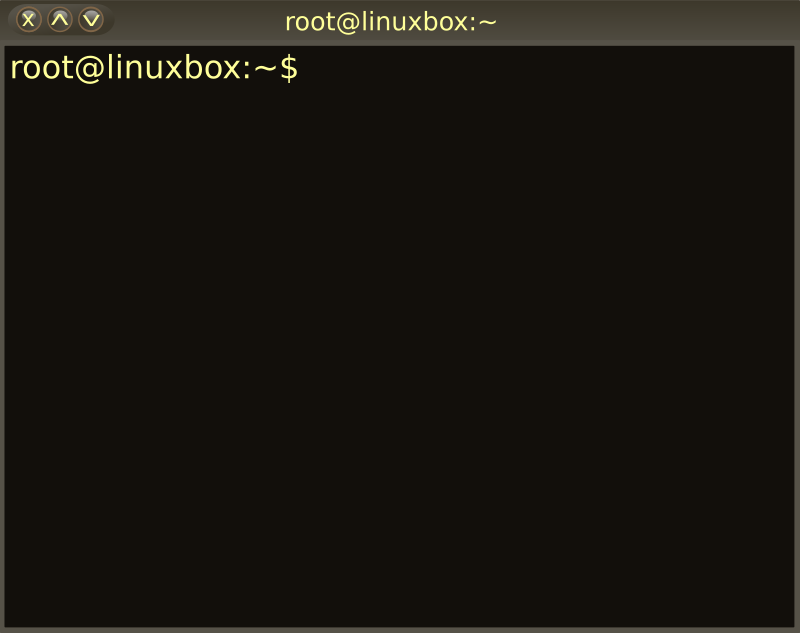
\includegraphics[width=\linewidth]{figures/lab1_1.png}
            \caption{Part 1, Console Output}
            \label{fig:part1_output}
        \end{figure}
